\documentclass[12pt,a4paper]{article}
\usepackage[utf8]{inputenc}
\usepackage[T1]{fontenc}
\usepackage{amsmath}
\usepackage{amsfonts}
\usepackage{amssymb}
\usepackage{ stmaryrd }
\usepackage{amsthm}
\usepackage{graphicx}
\usepackage{subfigure}
\usepackage{float}
\newtheorem*{lemma}{Lemma}
\newtheorem*{theorem}{Theorem}
\newtheorem*{corollary}{Corollary}
\newtheorem*{prf}{\textbf{Proof}}
\usepackage{caption}
\DeclareMathOperator{\n}{\nabla}
\DeclareMathOperator{\E}{\mathrm{E}}
\DeclareMathOperator{\xyz}{\textbf{numpy.random.normal()}}
\title{CS331-HW9-Lukang-Sun}
\begin{document}
	\maketitle
	\paragraph{p1.}
	(see Figure $\ref{img2}$.)
	a = [matrix([[0.1]]), matrix([[0.424466]]), matrix([[0.77981303]]), matrix([[0.20033184]]), matrix([[0.51116473]]), matrix([[0.2604399]]), matrix([[0.97100656]]), matrix([[0.21263449]]), matrix([[0.26417151]]), matrix([[0.15995097]])]
	
	b = [matrix([[0.4231786]]), matrix([[0.524466]]), matrix([[0.17981303]]), matrix([[0.50033184]]), matrix([[0.71116473]]), matrix([[0.0604399]]), matrix([[0.37100656]]), matrix([[0.91263449]]), matrix([[0.66417151]]), matrix([[0.65995097]])]
	,$f=\frac{1}{10}\sum_{i=1}^{10}f_i(x,y),f_i(x,y)=\sin(x+a[i])+\cos(y+b[i])$, for the SGD method, I use SGD-Uniform sampling.
		\begin{figure}
		\centering
		\subfigure[ ]{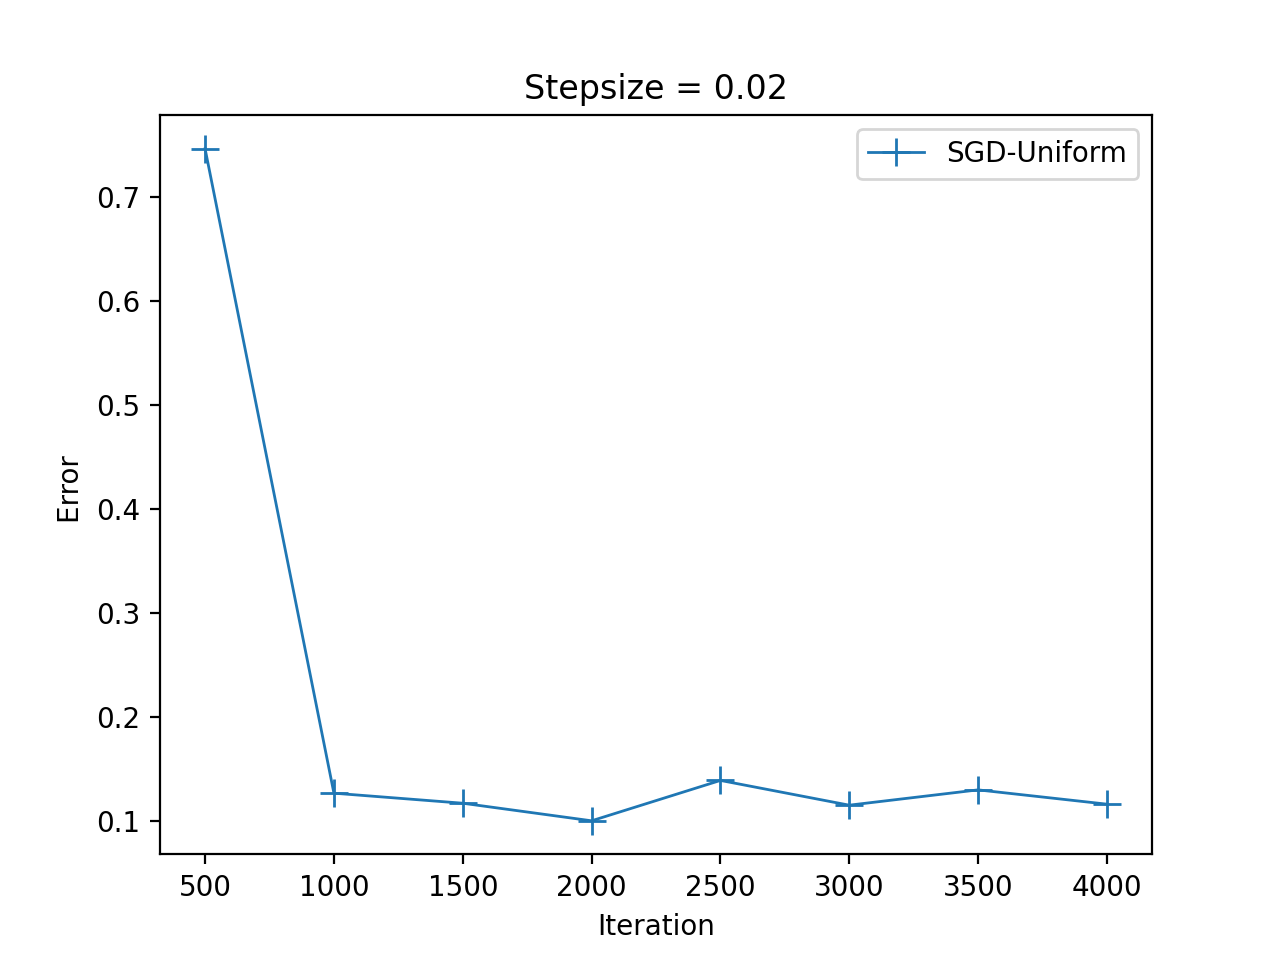
\includegraphics[width=6.7cm]{Figure_91.png}} 
		\subfigure[]{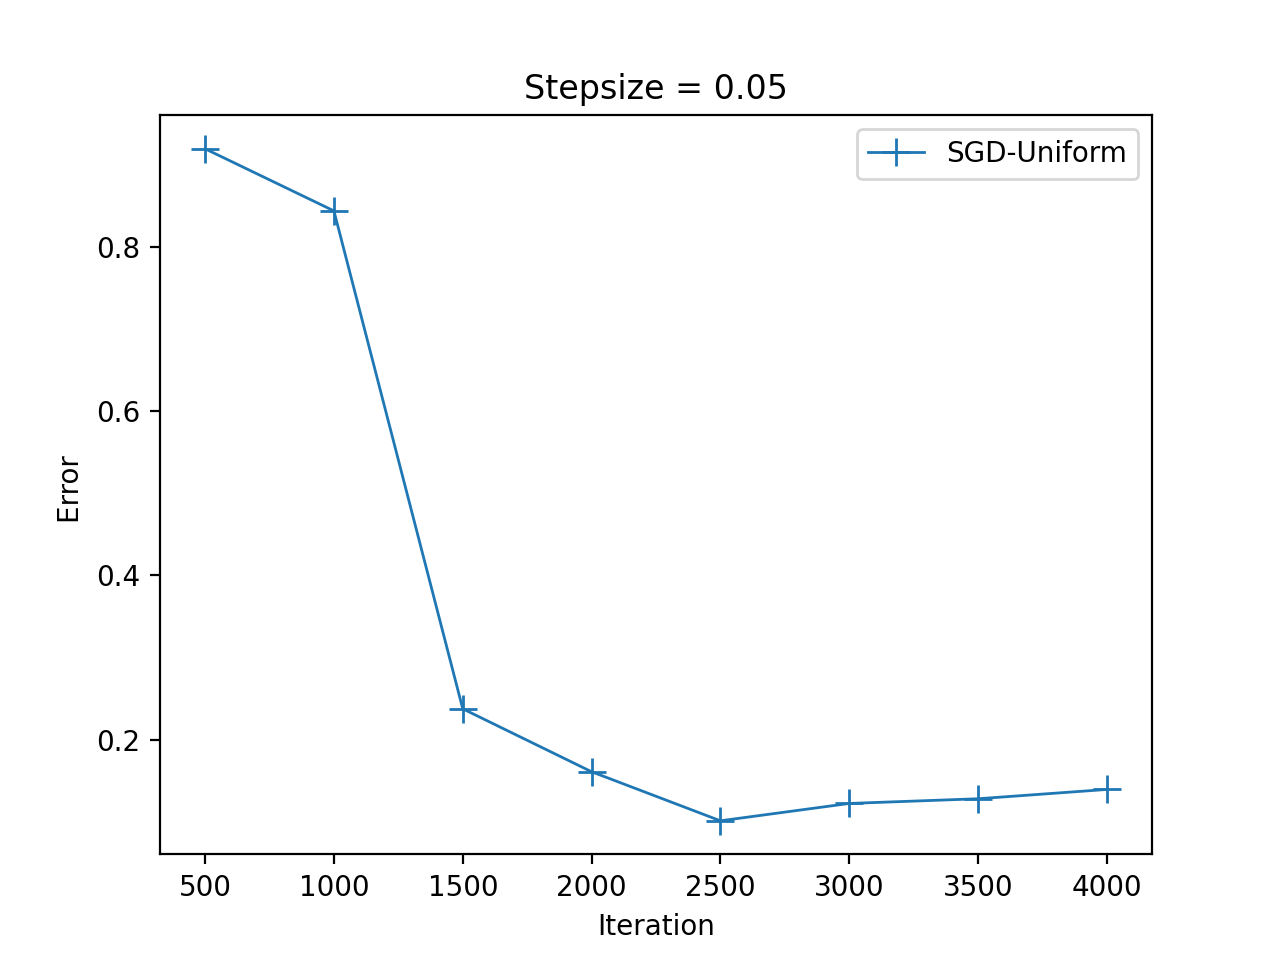
\includegraphics[width=6.7cm]{Figure_92.png}}
		
		
		\caption{ (a) shows $\E\left[||\nabla f||^2\right]$ changes in terms of iteration number K when set step size $\gamma = 0.02$,(b)  shows $\E\left[||\nabla f||^2\right]$ changes in terms of iteration number K when set step size $\gamma = 0.05$.} %图片标题
		\label{img2}
	\end{figure}
\newline
(i)each $f_i$ is at most 1-smoothness, since its Hessian is diagonal and bound by $diag(1,1)$, so $f$ is at most 1-smoothness, and it's obvious $f_i,f$ are not convex at all.  And this method satisfy $A B C-$ assumption, $\E\left[||g_i(x)||^2_2\right]\leq 2 A\left(f(x)-f^{\mathrm{inf}}\right)+B\|\nabla f(x)\|^{2}+C$, obviously, C is less 2 since $f_i,f$ bounded by 2, and we can set $A=0,B=0$( $\E\left[||g_i||^2_2\right]\leq 2$).
\newline
(ii) I test how the error change in terms of K and the step size. Since in this case, only step size $\gamma$ and $K$ influence the error.
\newline
(iii) First I set $\gamma$ fixed and change K. Then I set K fixed and change $\gamma$. By control one variable, we can clearly find the error change in terms of the other variable.
\newline
(iv)Theory states that the error change proportional to $\frac{1}{K}$ in certain error bound when $\gamma$ is small and fixed and proportional to $\gamma$ when K is fixed(generally very lage $>>\frac{1}{\gamma}$), these theory statements quite match my experiment results and my experiments shows the error change proportional to $\frac{1}{K}$ in certain error bound when $\gamma$ is small and fixed and proportional to $\gamma$ when K is fixed(generally very lage $>>\frac{1}{\gamma}$).
	

	\paragraph{p2.}
	\begin{lemma}
		Assume that $f$ is $\mu$-convex, $g^{t}$ is unbiased (Assumption 1) and that the $A C$ assumption (Assumption 2) is satisfied. Choose a stepsize satisfying
		$$
		0<\gamma_t \leq \frac{1}{A}
		$$
		Then the iterates $\left\{x^{t}\right\}_{t \geq 0}$ of SGD (Algorithm 3) satisfy
		$$
		\mathrm{E}\left[\left\|x^{t+1}-x^{\star}\right\|^{2}\right] \leq(1-\gamma_t \mu)\mathrm{E}\left[\left\|x^{t}-x^{\star}\right\|^{2}\right]+\gamma_t^2C
		$$
	\end{lemma}
	\begin{proof}
		the proof is exactly the  same as theorem 30
	\end{proof}
	\begin{lemma}
		Let $a, b, c \geq 0$ with $0<a \leq b$. Consider a sequence $\left\{d_{t}\right\}_{t \geq 0}$ satisfying
		$$
		d_{t+1} \leq\left(1-\gamma_{t} a\right) d_{t}+\gamma_{t}^{2} c
		$$
		where $\gamma_{t} \leq \frac{1}{b}$ for all $t \geq 0 .$ Fix $K>0$ and let $\theta=\left\lceil\frac{K}{2}\right\rceil$ and $s=\frac{2 b}{a} .$ Then choosing the stepsize as
		$$
		\gamma_{t}= \begin{cases}\frac{1}{b}, & \text { if } K \leq 2(s-1) \\ \frac{1}{b}, & \text { if } K>2(s-1) \text { and } t<\theta \\ \frac{2}{a(s+t-\theta)} & \text { if } K>2(s-1) \text { and } t \geq \theta\end{cases}
		$$
		gives
		$$
		d_{K} \leq \exp \left(-\frac{a K}{2 b}\right) d_{0}+\frac{12 c}{a^{2} K}
		$$
	\end{lemma}
	\begin{proof}
		this is exactly lemma 117.
	\end{proof}
	\begin{theorem}
		Assume that $f$ is $\mu$-convex, $g^{t}$ is unbiased(Assumption 1) and that the $A C$ assumption is satisfied. Choose the stepsize as 
		$$
		\gamma_{t}= \begin{cases}\frac{1}{A}, & \text { if } K \leq 2(s-1) \\ \frac{1}{A}, & \text { if } K>2(s-1) \text { and } t<\theta \\ \frac{2}{\mu(s+t-\theta)} & \text { if } K>2(s-1) \text { and } t \geq \theta\end{cases},
		$$
		where $K$ is any chosen integer, $\theta=\left\lceil\frac{K}{2}\right\rceil,s=\frac{2 A}{\mu},$
		then we have 
		$$
		\E\left[||x^K-x^{\star}||_2^2\right]\leq\exp\left(-\frac{\mu K}{2A}\right)||x^0-x^{\star}||^2+\frac{12C}{\mu^2K}
		$$
	\end{theorem}
	\begin{proof}
		this is an corollary of the last lemma.
	\end{proof}

	\paragraph{p3.}
	\begin{proof}
	(i)Let's assume $A$ is a matrix with full row rank.(if not,assume its row rank is l, then left multiply a $m\times m$ full rank matrix L,such that LA's first l row has full rank and the left row is 0, then we can do the same analysis in a affine subspace($\phi$ is strongly convex when constrained in a affine space $\left\{ Ax+b,x\in\mathbb{R}^d\right\}$). Further if $\phi(x)$ is strongly convex if and only if $\phi_{L}(x):=\phi(Lx)$ is strongly convex.Since it is easy to see that
	 $D_{\phi}(x,y)\geq \mu_1 ||x-y||_2^2\Longleftrightarrow D_{\phi_{L}}(x,y)\geq \mu_2 ||x-y||^2_2$ ). It's easy to verify that $f$ is convex
	 ($f(\lambda x+(1-\lambda)y)=\phi(\lambda(Ax+b)+(1-\lambda)(Ay+b))\leq \lambda \phi(Ax+b)+\lambda\phi((1-\lambda)(Ay+b))=\lambda f(x)+(1-\lambda)f(y)$,) so there is $x^{\star}$, such that $\nabla f(x^{\star})=A^T\nabla \phi(Ax^{\star}+b)=0$.
	 Due to $D_{\phi}(a,y)\leq C ||\nabla\phi(a)-\nabla \phi(y)||^2_2$, 
	 for any $a,y\in \mathbb{R}^m$, insert $a=Ax+b$ and $Ax^{\star}+b$, we get $f(x)-f(x^{\star})-\langle\nabla \phi(Ax^{\star}+b),A(x-x^{\star})\rangle\leq C
	  ||\nabla \nabla \phi(Ax+b)-\nabla \phi(Ax^{\star}+b)||^2_2=C||\nabla \phi(Ax+b)||^2_2$ since $A^T$ has full column rank $A^T\nabla\phi(A^{\star}+b)=0\Mapsto \phi(Ax^{\star}+b)=0$, where $\langle\nabla \phi(Ax^{\star}+b),A(x-x^{\star})\rangle(=\langle A^{T}\nabla \phi(x^{\star}), x-x^{\star}\rangle)=0$, so we have $f(x)-f(x^{\star})\leq C||\nabla \phi(Ax+b)||^2_2\leq CM||\nabla f(x)||^2_2$, where $M= \max_{x\in \mathbb{R}^m}\frac{||x||^2_2}{||A^Tx||^2_2}\leq +\infty$,since $A^T$ has full column rank.
	  \newline
	  (ii)$D_{\phi}(Ax+b,Ax^{\star}+b)\geq C_1||A(x-x^{\star})||^2_2\geq {C_1N}||x-x^{\star}||^2_2$, so we have $f(x)-f(x^{\star})\geq {C_1N}||x-x^{\star}|^2_2$, where
	  $N:=\min_{x\in\mathbb{R}^d}\frac{||Ax||^2_2}{||x||^2_2}$, $N$ could be 0. Actually, let $\phi=\frac{x^2}{2}, A=(1,0),b=0,$ then $f(x,y)=\frac{x^2}{2}$, $f(0,y)-f(0,0)=0=0||(0,y)-(0,0)||^2_2=0y^2.$
	  \end{proof}	
\end{document}